\documentclass[12pt,a4paper]{article}
\usepackage{tpl}
\dbegin{Кружок 7 класса, продолжающие, школа 179}{Решения занятия №14}

\z По кругу стоят $179$ корзин. Можно ли разложить в них яблоки так, чтобы в любых двух соседних корзинах число яблок отличалось на $2$?

\s Будем двигаться по кругу по часовой стрелке. Заметим, что количество раз, когда после перехода количество яблок увеличилось, должно быть равно количеству раз, когда оно уменьшилось. Но это значит, что количество переходов чётно, а оно $179$, т.е. разложить так яблоки нельзя. \QEDA\\

\z $15$ гномов собрали $100$ орехов. Докажите, что какие-то два из них собрали орехов поровну.

\s Пусть это не так. Тогда упорядочим их по возрастанию количества орехов, которое они собрали. После этого первый гном собрал хотя бы $0$ орехов, второй --- хотя бы $1$ орех, \ldots, $15$-й --- хотя бы $14$. Тогда собрано хотя бы $0+1+2+\ldots+14=105>100$ орехов, противоречие.\QEDA\\

\z Каждый день на рассвете из замка Перебор выезжает гонец и, проведя в пути две недели, прибывает в замок Идея. В тот же день он отправляется назад тем же маршрутом и, проведя в пути ещё две недели, к вечеру возвращается в Перебор. Сколько других гонцов повстречает он на пути?

\s На пути из Перебора в Идею первый гонец, встреченный нашим гонцом, отправился из Идеи за $14$ дней, а последний --- через $13$ дней относительно дня отбытия из Перебора. На пути из Идеи в Перебор первый встреченный гонец отправился за $13$ дней, а последний --- через $14$ дней относительно дня отбытия из Идеи. Всего таких гонцов $56$. \QEDA\\ 

\n С утра гном Хвалин отправляется к приятелю обсуждать новости. По пути он выходит на почтовый тракт, проходящий здесь точно по прямой, и поджидает гонца из Перебора, чтобы получить от него письмо. Где Хвалин должен выйти на тракт, чтобы его путь оказался самым коротким?\label{hvalin}

\s Если Хвалин и приятель живут по разные стороны от тракта, очевидно, что Хвалин должен пройти по прямой от своего дома до дома приятеля (\ref{hvalin1}). Если по одну, то нужно отразить дом приятеля относительно тракта и провести между отражением и домом Хвалина прямую. Вернём отражение назад и получим кратчайший путь (он кратчайший, потому что при отражении второй части пути мы придём в отражённый дом Хвалина, см. \ref{hvalin2}). \QEDA

\p Две деревни находятся по разные стороны от реки, берега которой – параллельные прямые. В каком месте реки необходимо построить мост, перпендикулярный берегам, чтобы путь из одной деревни в другую был минимален?\label{villages}

\s Представим, что реки нет, и сдвинем деревню 2 к реке на расстояние, равное ширине реки (см. \ref{villages1}, исходные деревни обозначены чёрными, образ --- красным). Пусть при этом получится деревня 2'. Тогда после пути мы пройдём какой-то путь между 1 и 2' и ещё ширину реки. Поэтому кратчайший путь получится, если провести отрезок между деревней 1 и деревней 2', пересечь его с ближним к 1 берегом реки и построить мост в этом месте. \QEDA

\begin{figure}[!htb]
	\begin{minipage}{0.32\textwidth}\centering
		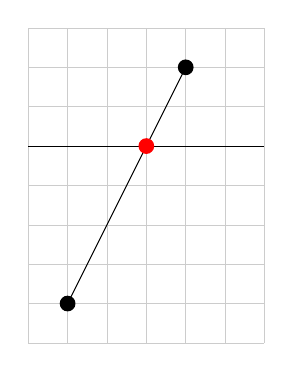
\begin{tikzpicture}
			\draw[step=0.5,very thin,black!20] (-0.5,-2.5) grid (2.5,1.5);
			\path[draw] (-0.5,0) -- (2.5,0);
			\fill (0,-2) circle[radius=0.1];
			\fill (1.5,1) circle[radius=0.1];
			\path[draw] (0,-2) -- (1.5,1);
			\fill[red] (1,0) circle[radius=0.1];
		\end{tikzpicture}
		\caption{\ref{hvalin}: первый случай}\label{hvalin1}
	\end{minipage}
	\begin{minipage}{0.32\textwidth}\centering
		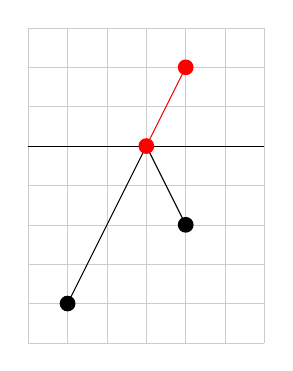
\begin{tikzpicture}
			\draw[step=0.5,very thin,black!20] (-0.5,-2.5) grid (2.5,1.5);
			\path[draw] (-0.5,0) -- (2.5,0);
			\fill (0,-2) circle[radius=0.1];
			\fill[red] (1.5,1) circle[radius=0.1];
			\fill (1.5,-1) circle[radius=0.1];
			\path[draw] (0,-2) -- (1,0) -- (1.5,-1);
			\fill[red] (1,0) circle[radius=0.1];
			\path[draw,red] (1,0) -- (1.5,1);
		\end{tikzpicture}
		\caption{\ref{hvalin}: второй случай}\label{hvalin2}
	\end{minipage}
	\begin{minipage}{0.32\textwidth}\centering
		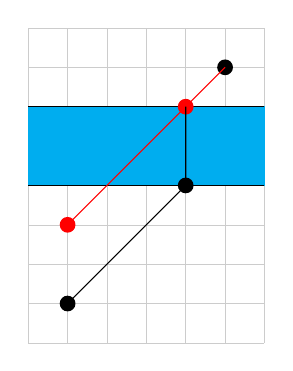
\begin{tikzpicture}
			\draw[step=0.5,very thin,black!20] (-0.5,-2.5) grid (2.5,1.5);
			\draw[fill,cyan] (-0.5,-0.5) -- (2.5,-0.5) -- (2.5,0.5) -- (-0.5,0.5) -- cycle;
			\path[draw] (-0.5,-0.5) -- (2.5,-0.5);
			\path[draw] (-0.5,0.5) -- (2.5,0.5);
			\fill (0,-2) circle[radius=0.1];
			\fill[red] (0,-1) circle[radius=0.1];
			\fill (2,1) circle[radius=0.1];
			\path[draw,red] (0,-1) -- (2,1);
			\fill[red] (1.5,0.5) circle[radius=0.1];
			\path[draw] (1.5,0.5) -- (1.5,-0.5) -- (0,-2);
			\fill (1.5,-0.5) circle[radius=0.1];
		\end{tikzpicture}
		\caption{\ref{villages}}\label{villages1}
	\end{minipage}
\end{figure}
\newpage

\z В ряд стоят $30$ кроссовок --- $15$ правых и $15$ левых. Докажите, что среди некоторых $10$ подряд стоящих кроссовок правых и левых поровну.

\s Рассмотрим количество левых кроссовок на разных промежутках из $10$ кроссовок. При смещении на $1$ кроссовок это число может измениться максимум на $1$. Если мы разделим ряд кроссовок на $3$ части по $10$, и ни в одной не ровно $5$ левых, есть две соседние части, в одной из которых больше $5$, а в другой --- меньше. Следовательно, где-то между ними есть $10$ подряд стоящих кроссовок, среди которых ровно $5$ левых. \QEDA\\

\z Улитка двигалась таким образом, что за каждый промежуток в одну минуту она проползла ровно один метр. Следует ли из этого, что она двигалась равномерно?

\s Нет, не следует. Например, улитка могла чередовать по полминуты движение со скоростью $2$ м/мин и нахождение на месте. \textit{Примечание. Подходит любой пример, где улитка повторяет свои движения каждую минуту, и при этом проползает за неё метр.}\QEDA\\

\z Двое играют на доске $10\times10$, за ход нужно положить на любые две соседние клетки доминошку так, чтобы доминошки не перекрывались. Проигрывает тот, кто не может сделать ход. Кто выиграет при правильной игре и как он должен играть, чтобы победить?

\s Второй выигрывает стратегией <<сделать ход, центрально-симметричный (относительно центра доски) последнему ходу первого>>. \QEDA\\

\z Имеется два бикфордовых шнура. При поджигании шнуры горят неравномерно, но каждый сгорает ровно за $20$ минут. Как с помощью этих шнуров отмерить $15$ минут? 

\s Одновременно подожжём один из них с обоих сторон, другой с одной стороны. Когда первый сгорит, пройдёт $10$ минут (т.к. если подождать ещё столько же времени, он бы сгорел два раза). После этого подожжём второй из них с другой стороны. Тогда через $5$ минут он догорит. \QEDA\\

\n Дано $2019$ целых чисел. Известно, что сумма любых $100$ из них положительна. Верно ли, что сумма всех чисел положительна?

\s Это верно. Действительно, отрицательных чисел не больше $99$ (иначе можно взять $100$ отрицательных чисел и их сумма отрицательна). Поместим их в одну сотню. Сумма этой сотни положительна, а всех оставшихся чисел неотрицательна, значит, сумма всех чисел положительна. \QEDA

\p $2019$ целых чисел стоят в ряд. Известно, что сумма любых $100$ последовательно стоящих чисел положительна. Верно ли, что сумма всех чисел положительна?

\s Это неверно. Приведем пример, когда это не так. Разделим $2019$ на <<комплекты>> по $19$ чисел и $81$ числу. Пусть в каждом из <<комплектов>> числа равны, сумма чисел в каждом из комплектов из $19$ чисел будет равна $-a$, а в каждом комплекте из $81$ числа будет равна $a+1$ (например, подойдёт, если в <<малых>> комплектах все числа $-17$, а в <<больших>> $4$). Теперь поставим их в таком порядке: $19,81,\ldots,19$.Тогда в каждой сотне сумма равна $1$, и при нашем выборе чисел общая сумма $-303<0$. \QEDA\\

\newpage
\n Есть $n$ камешков, различных по весу, и двухчашечные весы без гирь. Как за наименьшее число взвешиваний найти самый тяжелый камешек, если на весы можно класть только по одному камню?\footnote{\textit{Примечание.} На самом деле, ответ не меняется, если можно класть больше одного камня за раз. Это можно доказать так. Пусть веса камней --- $10-1,10-\frac12,10-\frac14,\ldots,10-2^{n-1}$. Тогда если класть разное количество камней на весы, то они будут показывать, где больше камней, а если одинаковое --- перевешивать будет чаша, где нет минимального камня из лежащих на весах. Пусть вместо взвешивания к нам будет подходить шпион и, если количество камней одинаково, будет показывать на минимальный камень, тогда мы получим заведомо не меньше информации. Тогда ясно, что меньше чем $n-1$ взвешиванием не обойтись.}

\s Нужно $n-1$ взвешивание. Возьмем любую пару камней, определим самый тяжелый из них. Самый тяжелый будем взвешивать с любым из невзвешенных камней. В полученной паре определяем самый тяжелый и снова взвешиваем с одним из невзвешенных. Повторяем это до тех пор, пока не взвесим все камни. Легко понять, что это оптимальный алгоритм. \QEDA

\p Есть $68$ камешков, различных по весу, и двухчашечные весы без гирь. Как за $100$ взвешиваний найти самый тяжёлый и самый лёгкий камни?

\s Разобьем все камни по парам и камни в каждой паре сравним между собой. На это мы потратим $34$ взвешивания. Самые тяжелые отложим в одну сторону, а самые легкие в другую. Теперь нам нужно $n-1$ взвешивание на каждую из кучек (по алгоритму из прошлого пункта), т.е. $33$ на каждую. На это мы потратим $34+66=100$ взвешиваний. \QEDA\\

\z Имеется $12$ одинаковых по виду монет, из которых одна фальшивая, отличающаяся по весу от настоящих, и двухчашечные весы без гирь. Как за наименьшее число взвешиваний найти фальшивую монету и узнать, легче она или тяжелее настоящих?

\s Минимальное количество взвешиваний --- $3$.

\textit{Оценка.} Даже если известно, что фальшивая монета легче настоящих, то за $2$ взвешивания можно обработать максимум $9$ монет (частный случай задачи, которая была на одном из предыдущих занятий). Значит, $2$ взвешиваний не хватит.

\textit{Алгоритм.} Первое взвешивание сделаем такое: разделим монеты на три кучи по четыре монеты (пусть это кучи из монет $1-4$, $5-8$, $9-12$) и взвесим первые две кучи. Тогда:

\begin{itemize}
	\item Пусть кучи равны по весу. Тогда у нас остались монеты $9-12$, одна из которых фальшивая, и $8$ заведомо настоящих монет. Взвесим $9,10$ и $11,1$. Если эти кучи равны, то фальшивая --- $12$ и можно за 1 взвешивание определить, легче она настоящих или тяжелее. Если нет, то либо $9$ или $10$ --- фальшивая тяжёлая, либо $11$ --- фальшивая лёгкая. Взвесим $9,11$ и $1,2$. Пусть в 2-м взвешивании перевесила кучка $9,10$ (иначе аналогично, но <<легче>> и <<тяжелее>> поменяем местами, а <<больше>> заменим на <<меньше>>). Тогда
	\begin{itemize}
		\item Если $9,11$ больше, то $9$ --- фальшивая тяжёлая.
		\item Если $1,2$ больше, то $11$ --- фальшивая лёгкая.
		\item Если они равны, то $10$ --- фальшивая тяжёлая.
	\end{itemize}
\item Пусть куча $1-4$ перевесила кучу $5-8$. Тогда сравним $1,2,5,9$ с $3,6,7,10$. Если они равны, то либо $4$ --- фальшивая тяжёлая, либо $8$ --- фальшивая лёгкая, и сравнением $4$ с $12$ это можно определить. Иначе пусть первая из этих $2$ куч перевесила (иначе аналогично). Это значит, что либо $1$ или $2$ фальшивая тяжёлая, либо $3$ --- фальшивая лёгкая, и мы умеем различать эти случаи за $1$ взвешивание (см. предыдущий пункт).\QEDA\\
\end{itemize}

\end{document}
